%%%%%%%%%% NO OLVIDAR COLOCAR ESTE COMENTARIO CON EL NUMERO DE EJERCICIO %%%%%%%%%%%%%
%%%%%%%%%%%%%%%%%%% EJERCICIO 7 %%%%%%
%%Text bf para negrilla , el \\ es para el salto de linea.
%%El primer \\ hace un espacio en el texto y el 2 \\ crea otro espacio
\textbf{Ejemplo 6}\newline
Una persona necesita tener reunidos 100.000 COP para el día 15-10-95, para tal fin constituye un fondo mediante depósitos trimestrales de R efectuándose el primero el día 15-7-90 y el último el 15-4-95 además se efectuará un depósito extraordinario de 8.000 COP el 15-1-93. Si el fondo paga el 24\% nominal anual trimestre vencido. ¿Cuál es el valor de la cuota de la serie uniforme? Considerar un año de 360 días.\\ \\

\textbf{Solución.}\\
\begin{center}

 \renewcommand{\arraystretch}{1.5}% Margenes de las celdas
 %Creación de la cuadricula
 \begin{tabular}{|c|c|c| }
  %Creamos una linea horizontal
  \hline
  %Definimos el color de la primera fila
  \rowcolor[HTML]{FFB183}
  %%%%% INICIO ASIGNACIÓN FECHA FOCAL %%%%%%%
  %%%%%%%%%% INICIO TITULO
  %Lo que se hace aquí es mezclar las 3 columnas en una sola
  \multicolumn{3}{|c|}{\cellcolor[HTML]{FFB183}\textbf{1. Asignación período focal}}                             \\ \hline
  %%%%%%%%%% FIN TITULO
  %%%%% INICIO DECLARACIÓN DE VARIABLES %%%%%%%
  \multicolumn{3}{|c|}{$pf = 0 ptv$}                                                                           \\ \hline
  %Definimos el color de la primera fila
  \rowcolor[HTML]{FFB183}
  %%%%% INICIO DECLARACIÓN DE VARIABLES %%%%%%%
  %%%%%%%%%% INICIO TITULO
  \multicolumn{3}{|c|}{\cellcolor[HTML]{FFB183}\textbf{2. Declaración de variables}}                           \\ \hline
  %%%%%%%%%% FIN TITULO
  %%%%%%%%%% INICIO DE MATEMÁTICAS
  VF= 100.000 COP                                        & $P_{3}=$ 8.000 COP                   & $j=24\% natv\equiv 6\% ptv =i$   \\\hline
  $n_{1}=20$ ptv                    & $n_{2}=2 $ ptv                    & $n_{3}=11 $ ptv  \\\hline
  \multicolumn{3}{|c|}{$R_{1}= ? COP $}                   \\ \hline

  %%%%%%%%%% FIN DE MATEMÁTICAS
  %%%%% FIN DECLARACIÓN DE VARIABLES


  %%%%% INICIO FLUJO DE CAJA
  \rowcolor[HTML]{FFB183}
  \multicolumn{3}{|c|}{\cellcolor[HTML]{FFB183}\textbf{3. Diagrama de flujo de caja}}                          \\ \hline
  %Mezclamos 3 columnas y pondremos el dibujo
  %%%%%%%%%%%%% INSERCIÓN DE LA IMAGEN
  \multicolumn{3}{|c|}{ 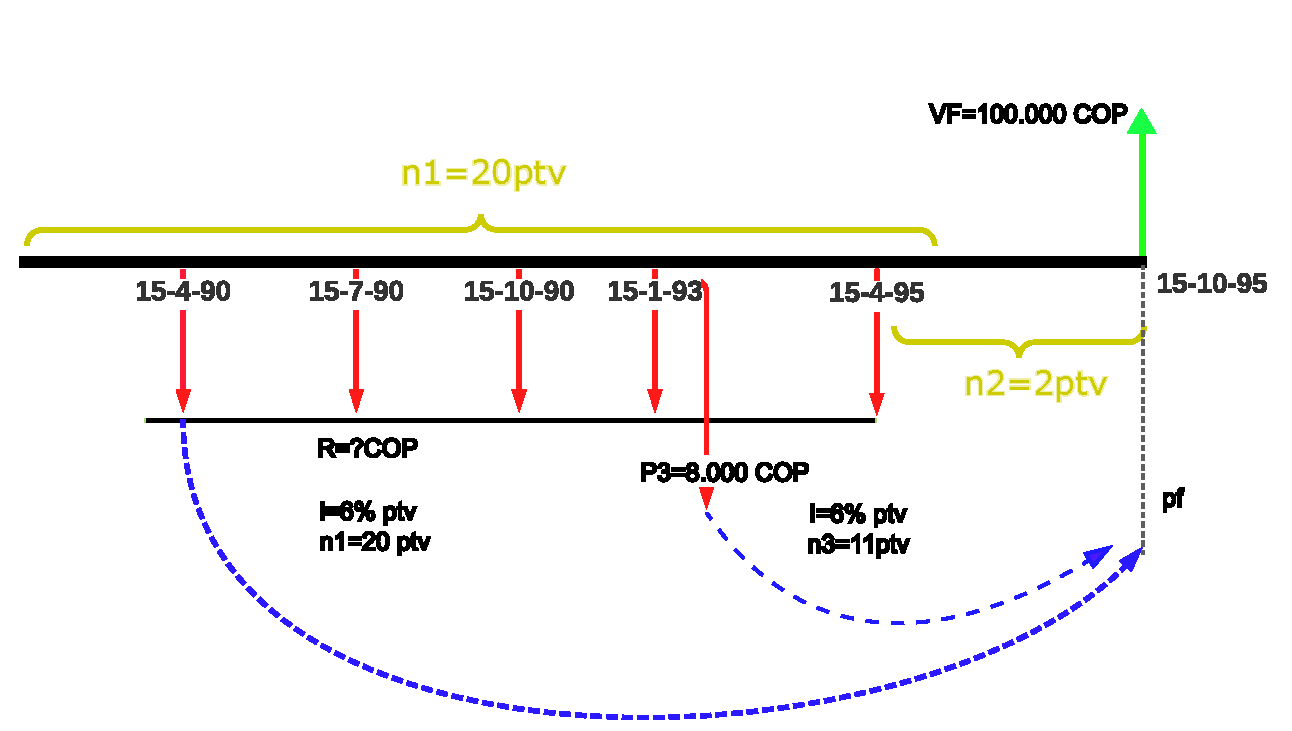
\includegraphics[width=0.9\columnwidth]{4_Capitulo/img/ejemplos/7/capitulo4ejemplo7.pdf} }   \\ \hline
  %%%%%%%%%%%%% FIN INSERCIÓN DE IMAGEN
  %%%%%FIN FLUJO DE CAJA



  %%%%% INICIO DECLARACIÓN FORMULAS
  %%%%%%%%%%% INICIO TITULO
  \rowcolor[HTML]{FFB183}
  \multicolumn{3}{|c|}{\cellcolor[HTML]{FFB183}\textbf{4. Declaración de fórmulas}}                            \\ \hline
  %%%%%%%%%%% FIN TITULO
  %%%%%%%%%%% INICIO MATEMÁTICAS

  \multicolumn{3}{|c|}{$VF = R \frac{((1+i)^{n}-1)}{i} F = P(1+i)^{n} {i}$ Valor futuro serie uniforme vencida} \\ \hline
  %%%%%%%%%% FIN MATEMÁTICAS
  %%%%%% INICIO DESARROLLO MATEMÁTICO
  \rowcolor[HTML]{FFB183}
  %%%%%%%%%%INICIO TITULO
  \multicolumn{3}{|c|}{\cellcolor[HTML]{FFB183}\textbf{5. Desarrollo matemático}}                              \\ \hline
  %%%%%%%%%% FIN TITULO
  %%%%%%%%%% INICIO MATEMÁTICAS
  \multicolumn{3}{|c|}{$R_{1}(\frac{((1+0,06)^{20}-1)}{0,06})*(1+0,06)^{2}+$ 8.000 COP $(1+0,06)^{11}=$100.000 COP} \\ \hline
  %%%%%%%%%% FIN MATEMÁTICAS
  %%%%%% FIN DESARROLLO MATEMÁTICO

  \rowcolor[HTML]{FFB183}
  \multicolumn{3}{|c|}{\cellcolor[HTML]{FFB183}\textbf{6. Respuesta}}                                          \\ \hline

  \multicolumn{3}{|c|}{El valor de la cuota es de 2.051,99 COP}                                                                         \\ \hline
 \end{tabular}
 %Se crean dos lineas en blanco para que no quede el siguiente texto tan pegado
 \newline \newline
\end{center}
%%%%%%%%%%%%%%%%%%%%%%%%%%FIN EJERCICIO X %%%%%%%%%%%%%%%%%%%%%%%%%%%
